\chapter{Društvene mreže i zajednice}

Društvene mreže može se pronaći gdje god postoji sustav koji sadrži entitete koji su međusobno povezani. Primjera je mnogo, a neki od njih su: društvene web platforme, email mreža, web stranice koje sadrže poveznice prema dugima, uređaji koji su povezani preko internetske mreže i slično. 
Kako bi se skupina entiteta mogla nazvati društvenom zajednicom među njima mora postojati nekakav tip odnosa. Može biti jednosmjerni ili dvosmjerni te mogu postojati težine kojima se odnosu daje veća ili manja značajnost. Društvene mreže imaju složenu organizacijsku strukturu te se može pretpostaviti svojstvo lokalnosti koje kaže da ako jedan entitet ima veze prema neka druga dva entiteta onda je vjerojatnost da ta druga dva entiteta imaju vezu veća od prosječne. 

Društvene mreže imaju karakteristično svojstvo grupiranja u strukturu zajednice. Ako se čvorovi mreže mogu podijeliti u nepreklapajuće ili preklapajuće zajednice tako da broj veza između članova zajednice značajno premašuje broj veza između bilo koje dvije zajednice znači da mreža ima strukturu društvenih zajednica. Mreže koje imaju takvu strukturu često se mogu prikazati i kao hijerarijske strukture. U ovom radu obradit će se mreže koje sadrže nepreklapajuće strukture sa vezama koje nemaju određene težine.

Proces pronalaska društvenih zajednica jedan je od glavnih zadataka u analizama društvenih mreža. Detekcija zajednica može biti vrlo korisna u raznim primjenama kao što je primjerice pronalaženje grupa kojima bi se mogle slati reklame za određene proizvode koji bi ih mogli zanimati umjesto da se svakom pojedincu šalju posebno. Još jedan primjer bio bi preporuka određenih sadržaja koji bi se mogli prikazivati grupama koje pokazuju zanimanja prema sličnim interesima. Primjera ima još mnogo, ali iz ova dva je već vidljivo da se korisne informacije mogu zaključivati iz društvenih mreža. Kako bi društvene mreže pohranili i analizirali u računalu potrebna je prikladna struktura podataka koja će u ovom slučaju biti graf.

\section{Reprezentacija društvenih mreža}
Prema definiciji jednostavan graf \textit{G} sastoji se od nepraznog konačnog skupa \textit{V(G)}, čije se elemente naziva vrhovi ili čvorovi grafa i konačnog skupa \textit{E(G)} različitih dvočlanih podskupova skupa \textit{V(G)} koji se naziva bridovima \cite{nakic_pavcevic_2019}. Graf može imati najviše $ {n(n-1) \over 2} $. U radu će se razmatrati jednostavni grafovi koji nemaju petlje i više bridova između istih čvorova. Bridovi će biti bestežinski i neusmjereni. 

Bitna definicija tiče se stupnja vrhova grafa. Stupanj vrha \textit{v} grafa \textit{G} je broj bridova koji su incidentni s \textit{v}. Stupanj vrha označava se sa \textit{deg(v)}. Vrh stupnja 0 zove se izolirani vrh, a vrh stupnja 1 krajnji vrh. \cite{nakic_pavcevic_2019}

Šetnja je graf sa skupom vrhova \textit{V(G) = $ \{x_{1},x_{2},...,x_{l}\} $ } i bridova \textit{E(G) = $ \{x_{0}x_{1},x_{1}x_{2},...,x_{l-1}x_{l}\} $ }. vrhovi $ x_{0} $ i $ x_{l} $ definiraju se kao krajevi dok je \textit{l} duljina šetnje. Ako su svi bridovi šetnje različiti tada se ona naziva staza. Ako su uz to i svi vrhovi različiti onda se takva šetnju naziva putem. Ako put počinje i završava u istom vrhu tada graf sadrži ciklus. Uz pretpostavljena ograničenja najmanji ciklus koji graf u ovom radu može imati je trokut što je često obilježje društvenih mreža.

Definicija puta omogućava definiranje važnog koncepta koji će se pojavljivati u radu pojedinih algoritama. Ako u grafu za svaki par vrhova postoji barem jedan put koji ide od jednog do drugog onda je graf povezan. Ako između vrhova postoji više putova onda je najkraći onaj koji ima najmanju duljinu. Promjer povezanog grafa je najveća udaljenost između bilo koja dva vrha u grafu. Ako ipak postoji barem jedan par vrhova između kojih ne postoji put onda je graf podijeljen u barem dva podgrafa. Svaki maksimalno povezani podgraf zove se komponenta povezanosti. Primjer se može vidjeti na slici \ref{fig:graph}.

\begin{figure}
	\makebox[\textwidth][c]{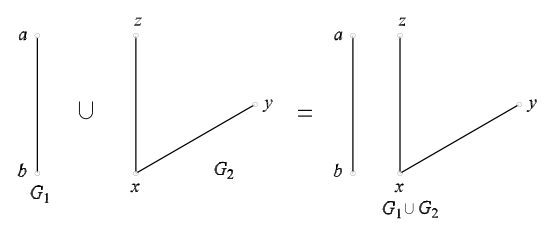
\includegraphics[width=0.7\textwidth]{images/nepovezani-graf.png}}
	%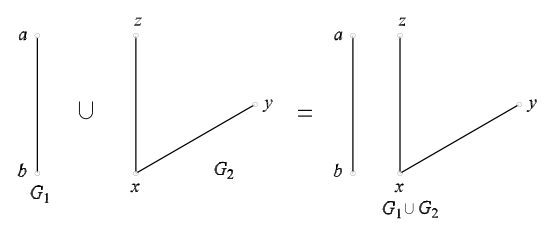
\includegraphics[width=0.7\textwidth]{images/nepovezani-graf.png}
	\caption{Primjer nepovezanog grafa}
	\label{fig:graph}
\end{figure}

Grafovi se mogu pohranjivati u obliku matrice susjedstva gdje su dva vrha, \textit{i} i \textit{j} susjedna ako im je element matrice \textit{A{ij}} jednak 1, a inače 0. Zbog pretpostavke da ne postoje petlje na dijagonali matrice susjedstva svi su elementi nule. Za reprezentaciju neusmjerenog grafa matrica susjedstva je simetrična što znači da je dovoljno pohraniti samo jedan trokut matrice, iznad ili ispod dijagonale. Suma elemenata \textit{i}-tog retka ili stupca jednaka je stupnju vrha \textit{i}

Jednostavniji oblik pohrane koji zauzima manje prostora u datoteci je takav da se pohranjuje popis bridova grafa te se i on može koristiti.


\section{Obilježja društvenih zajednica} 
